\chapter{Esperimenti}

\section{Introduzione}
In questo capitolo vengono presentati e analizzati in dettaglio i risultati degli esperimenti introdotti nel capitolo precedente, con l'obiettivo di valutare le prestazioni e l'efficacia dei diversi algoritmi di ottimizzazione applicati al training di reti neurali Multi-Layer Perceptron (MLP).
La sperimentazione è stata condotta seguendo una metodologia rigorosa e sistematica, al fine di garantire la comparabilità dei risultati e la validità delle conclusioni tratte. Gli esperimenti sono stati progettati per esplorare diverse dimensioni del problema di ottimizzazione: l'impatto della quantità di dati di training, l'influenza del numero di epoche, l'efficacia di approcci ibridi e i benefici della parallelizzazione.

\section{Allenamento con SGDM}
 L'allenamento della rete neurale MLP con SGDM, variando il numero di dati di training, ha generato i risultati mostrati in tabella. 
\begin{table}[htbp]
\centering
\begin{tabular}{|c|c|c|c|c|}
\hline
\textbf{Dati Training} & \textbf{Accuracy} & \textbf{Loss} & \textbf{Tempo (s)} & \textbf{Epoche} \\
\hline
1000 & 87.44\% & 0.436481 & 1.84 & 25 \\
\hline
5000 & 93.96\% & 0.236183 &  8.65 & 25 \\
\hline
10000 & 95.97\% & 0.153752 & 17.51 & 25 \\
\hline
15000 & 96.84\% &  0.115814 &28.69 & 25 \\
\hline
\end{tabular}
\label{tab:sgdm_results con 25 epoche}
\caption{Risultati allenamento SGDM con 25 epoche}
\end{table}

\newpage
Nella seguente tabella sono mostrati i risultati aumentando il numero di epoche a 100.
\begin{table}[htbp]
\centering
\begin{tabular}{|c|c|c|c|c|}
\hline
\textbf{Dati Training} & \textbf{Accuracy} & \textbf{Loss} & \textbf{Tempo (s)} & \textbf{Epoche} \\
\hline
1000 & 88.85\% & 0.581697 & 7.45 & 100 \\
\hline
5000 & 94.30 \% & 0.299773 &  36.93 & 100 \\
\hline
10000 & 96.14\% & 0.188318 & 75.97 & 100 \\
\hline
15000 & 96.94\% &  0.143579 & 112.85 & 100 \\
\hline
\end{tabular}
\label{tab:sgdm_results con 100 epoche}
\caption{Risultati allenamento SGDM con 100 epoche}
\end{table}

\section{Allenamento con GA}
    L'allenamento della rete neurale MLP con i GA, con vari metodi di crossover, utilizzando un numero di dati di training pari a 1000, ha generato i risultati mostrati in tabella.
    Come già detto precedentemente il numero di dati di training è stato scelto pari a 1000, in quanto l'allenamento con GA risulta essere molto più lento rispetto a SGDM, ADAM e le loro versioni ibride.
    Per questo motivo si è deciso di utilizzare un numero di dati di training più piccolo, per poter fare un confronto con gli altri metodi. Ovviamente questo comporta che bisogna confrontare i risultati
    ottenuti con GA con quelli ottenuti con SGDM con 1000 dati di training.
\begin{table}[htbp]
\centering
\begin{tabular}{|c|c|c|c|c|c|c|}
\hline
\textbf{Dati Train} & \textbf{Cross.} & \textbf{Accuracy} & \textbf{Loss} & \textbf{Tempo (h)} & \textbf{Gen.} & \textbf{Pop.} \\
\hline
1000 & Aritmetico & 66\% & 1.3410 & 2.5 & 250 & 100 \\
\hline
1000 & Blend & 74.90\% & 1.1595 & 2.5 & 250 & 100 \\
\hline
1000 & SBX & 58\% & 1.3022 & 2.5 & 250 & 100 \\
\hline
1000 & Adattivo & 70.20\% & 1.0636 & 2.5 & 250 & 100 \\
\hline
\end{tabular}
\label{tab:GA_results}
\caption{Risultati allenamento GA}
\end{table}
    Da questi esperimenti si può notare come il metodo di crossover più efficace sia stato il crossover blend, che ha portato ad una accuratezza del 74.90\% e una loss di 1.1595.
    C'è comunque da considerare, che seppur avendo tenuto lo stesso seed per tutti gli esperimenti, il GA è un algoritmo stocastico e quindi i risultati possono variare leggermente ad ogni esecuzione.
    Comunque si può notare come il GA non riesce a raggiungere le prestazioni di SGDM con 1000 dati di training, che ha portato ad una accuratezza dell'87.44\% e una loss di 0.436481.
    Questo è dovuto al fatto che il GA è un algoritmo di ottimizzazione globale, che cerca di esplorare tutto lo spazio delle soluzioni, ma non è molto efficace nel trovare soluzioni locali ottimali.
    Inoltre il tempo di allenamento è molto più lungo rispetto a SGDM, come si può notare dalla tabella, dove il tempo di allenamento con GA è di circa 2 ore, mentre con SGDM è di pochi secondi.
    Da ora in poi, per gli esperimenti con GA, si utilizzerà il crossover blend, essendo il metodo che ha prodotto i risultati migliori.
\section{Allenamento con GA parallelizzato}
    L'implementazione della parallelizzazione per l'allenamento della rete attraverso algoritmi genetici (GA) ha prodotto significativi miglioramenti in termini di efficienza computazionale, come evidenziato dai risultati presentati nella tabella seguente.
    La strategia di parallelizzazione adottata prevede l'utilizzo di otto processi simultanei, corrispondenti al numero di core logici del calcolatore utilizzato per la sperimentazione. Questa configurazione rappresenta il punto di equilibrio ottimale tra sfruttamento delle risorse hardware disponibili e prevenzione della contesa eccessiva per le risorse di sistema.
\begin{table}[htbp]
\centering
\begin{tabular}{|c|c|c|c|c|c|c|}
\hline
\textbf{Dati Train.} & \textbf{Cross.} & \textbf{Accuracy}& \textbf{Tempo (s)} & \textbf{Gen.} & \textbf{Pop.} & \textbf{Parallel.}\\
\hline
1000 & Blend & 66.68\%  & 7662.46 & 200 & 100 & No\\
\hline
1000 & Blend & 66.84\%  & 4637.13s & 200 & 100 & Si\\
\hline
\end{tabular}
\label{tab:GA_results}
\caption{Risultati allenamento GA}
\end{table}

    I dati sperimentali dimostrano chiaramente l'efficacia della parallelizzazione nell'ottimizzazione del processo di training. La versione parallelizzata dell'algoritmo ha conseguito una riduzione del tempo di esecuzione da 7662.46 secondi (circa 2.13 ore) a 4637.13 secondi (circa 1.29 ore), corrispondente a un miglioramento delle prestazioni del 39.5\% circa, mantenendo sostanzialmente invariata l'accuratezza del modello.
    L'efficacia della parallelizzazione è strettamente legata alle caratteristiche dell'architettura hardware utilizzata. L'impiego di otto processi paralleli, ha garantito un utilizzo ottimale delle risorse computazionali. È importante sottolineare che l'incremento del numero di processi oltre la capacità fisica del sistema tenderebbe a produrre un peggioramento delle prestazioni a causa della competizione per le risorse condivise.
    I risultati ottenuti suggeriscono un significativo potenziale di miglioramento delle prestazioni su architetture hardware più potenti. L'utilizzo di sistemi multi-core con un maggior numero di unità di elaborazione parallele potrebbe portare a riduzioni ancora più sostanziali dei tempi di training, sfruttando la natura intrinsecamente parallela degli algoritmi genetici.

\section{Allenamento con GASGDM}
    In questa sezione vengono presentati i miglioramenti ottenuti dall'utilizzo combinato di Algoritmo Genetico (GA) e Stochastic Gradient Descent with Momentum (SGDM), rispetto all'impiego del solo SGDM. 
    I test sono stati eseguiti su diverse partizioni del dataset, considerando set di training composti da 1.000, 5.000, 10.000 e 15.000 istanze. 
    I miglioramenti sono riportati nelle tabelle seguenti. È importante sottolineare che l'uso di GASGDM comporta un tempo di training maggiore rispetto al solo SGDM; tuttavia, questo è giustificato dal fatto che GASGDM è in grado di trovare soluzioni che SGDM non riuscirebbe a individuare nemmeno aumentando significativamente il numero di epoche.
    Per questi esperimenti sono stati scelti i seguenti parametri per GA e SGDM:
    \begin{compactitemize}
        \item \textbf{Numero di generazioni}: 10
        \item \textbf{Popolazione}: 10
        \item \textbf{Numero di cicli GASGDM}: 3
        \item \textbf{Epoche SGDM}: 10
    \end{compactitemize}


\begin{table}[htbp]
\centering
\begin{tabular}{|c|c|c|c|c|}
\hline
\textbf{Dati Train.} & \textbf{Metodo} & \textbf{Accuracy} & \textbf{Tempo (s)} & \textbf{Epoche SGDM} \\
\hline
1000 & SGDM & 88.80\% & 3.64 & 50 \\
\hline
1000 & GASGDM & 89.51\% & 79.23 & 10 \\
\hline
\end{tabular}
\caption{Risultati dell'allenamento con GASGDM su 1.000 istanze di training}
\label{tab:GASGDM_results_1000}
\end{table}

\begin{table}[htbp]
\centering
\begin{tabular}{|c|c|c|c|c|}
\hline
\textbf{Dati Train.} & \textbf{Metodo} & \textbf{Accuracy} & \textbf{Tempo (s)} & \textbf{Epoche SGDM} \\
\hline
5000 & SGDM & 94.33\% & 18.17 & 50 \\
\hline
5000 & GASGDM & 95.00\% & 174.52 & 10 \\
\hline
\end{tabular}
\caption{Risultati dell'allenamento con GASGDM su 5.000 istanze di training}
\label{tab:GASGDM_results_5000}
\end{table}

\begin{table}[htbp]
\centering
\begin{tabular}{|c|c|c|c|c|}
\hline
\textbf{Dati Train.} & \textbf{Metodo} & \textbf{Accuracy} & \textbf{Tempo (s)} & \textbf{Epoche SGDM} \\
\hline
10000 & SGDM & 96.11\% & 22.21 & 50 \\
\hline
10000 & GASGDM & 96.37\% & 315.38 & 10 \\
\hline
\end{tabular}
\caption{Risultati dell'allenamento con GASGDM su 10.000 istanze di training}
\label{tab:GASGDM_results_10000}
\end{table}


\begin{table}[H]
    \centering
    \begin{tabular}{|c|c|c|c|c|}
    \hline
    \textbf{Dati Train.} & \textbf{Metodo} & \textbf{Accuracy} & \textbf{Tempo (s)} & \textbf{Epoche SGDM} \\
    \hline
    15000 & SGDM & 96.90\% & 33.60 & 50 \\
    \hline
    15000 & GASGDM & 96.96\% & 442.14 & 10 \\
    \hline
    \end{tabular}
    \caption{Risultati dell'allenamento con GASGDM su 15.000 istanze di training}
    \label{tab:GASGDM_results_15000}
    \end{table}
    Per valutare la capacità di GASGDM di superare i minimi locali dello SGDM, è stato eseguito un esperimento incrementando il numero di epoche di SGDM a 300 e 500, mentre il numero di cicli GASGDM è stato aumentato a 6 e le epoche SGDM a 20.
\begin{table}[H]
    \centering
    \begin{tabular}{|c|c|c|c|c|}
    \hline
    \textbf{Dati Train.} & \textbf{Metodo} & \textbf{Accuracy} & \textbf{Tempo (s)} & \textbf{Epoche SGDM} \\
    \hline
    15000 & SGDM & 97.00\% & 465.55 & 300 \\
    \hline
    15000 & SGDM & 97.00\% & 771.12 & 500 \\
    \hline
    15000 & GASGDM & 97.06\% & 1484 & 20 \\
    \hline
    \end{tabular}
    \caption{Confronto tra SGDM e GASGDM su 15.000 istanze con epoche SGDM aumentate}
    \label{tab:GASGDM_results2_15000}
    \end{table}
    Dai risultati ottenuti emerge come l'efficacia dei metodi basati sul gradiente aumenti con l'incremento del numero di dati di training, consentendo di raggiungere buone soluzioni in tempi relativamente brevi. 
    Tuttavia, è importante sottolineare che GASGDM riesce a individuare soluzioni migliori rispetto al solo SGDM anche con un numero ridotto di epoche, dimostrando la sua capacità di superare minimi locali e ottimizzare in maniera più efficace.


\begin{figure}[htbp]
    \centering
    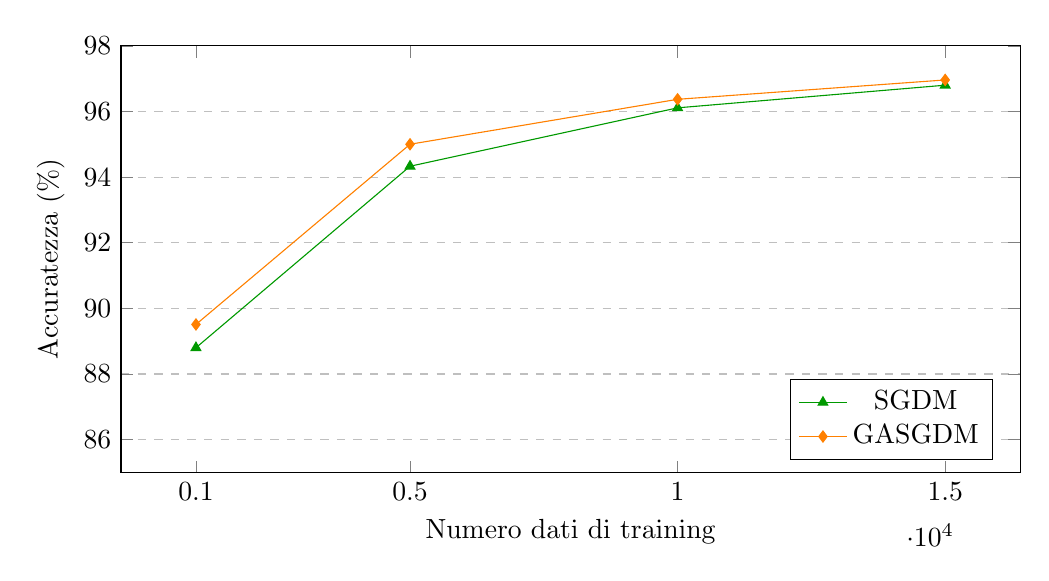
\begin{tikzpicture}
    \begin{axis}[
        width=13cm,
        height=7cm,
        xlabel={Numero dati di training},
        ylabel={Accuratezza (\%)},
        ymin=85, ymax=98,
        xtick={1000,5000,10000,15000},
        legend pos=south east,
        ymajorgrids=true,
        grid style=dashed
    ]
    
    % SGDM
    \addplot[
        color=green!60!black,
        mark=triangle*
    ] coordinates {
        (1000,88.80) (5000,94.33) (10000,96.11) (15000,96.80)
    };
    \addlegendentry{SGDM}
    
    % GASGDM
    \addplot[
        color=orange,
        mark=diamond*
    ] coordinates {
        (1000,89.51) (5000,95.00) (10000,96.37) (15000,96.96)
    };
    \addlegendentry{GASGDM}
    
    \end{axis}
    \end{tikzpicture}
    \caption{Accuratezza di SGDM vs GASGDM al variare della dimensione del dataset}
    \end{figure}
    
\section{Allenamento con GADAM}
    In questa sezione sono mostrati i miglioramenti ottenuti combinando GA e ADAM, che hanno permesso di trovare soluzioni migliori rispetto all’utilizzo del solo ADAM. I test sono stati fatti su 
    varie partizioni di dataset, in particolare è stato testato il comportamento su 1000, 5000, 10000 e 15000 istanze di training.
    I miglioramenti sono mostrati in tabella, ovviamente c'è da considerare il tempo maggiore per fare il training con GADAM, ciò è giustificato dal fatto che GADAM riesce a trovare soluzioni che altrimenti sarebbero impossibili da ottenere.
    Per fare questi esperimenti si è deciso di utilizzare i seguenti parametri per il GA e SGDM:
    \begin{compactitemize}
        \item \textbf{Numero di generazioni}: 10
        \item \textbf{Popolazione}: 5
        \item \textbf{Numero cicli GADAM}: variabile in base al numero di dati di training
        \item \textbf{Epoche ADAM}: 50
    \end{compactitemize}

\begin{table}[H]
\centering
\begin{tabular}{|c|c|c|c|c|c|}
\hline
\textbf{Dati Train.} & \textbf{Metodo} & \textbf{Accuracy}& \textbf{Tempo (s)} & \textbf{Epoche GADAM}\\
\hline
1000 & ADAM & 90.30\%  & 0.52 & 50 \\
\hline
1000 & GADAM &  90.67\%  & 77.13 & 50\\
\hline
\end{tabular}
\label{tab:GADAM_results_1000}
\caption{Risultati allenamento GADAM con 1000 istanze di training}
\end{table}


\begin{table}[htbp]
\centering
\begin{tabular}{|c|c|c|c|c|c|}
\hline
\textbf{Dati Train.} & \textbf{Metodo} & \textbf{Accuracy}& \textbf{Tempo (s)} & \textbf{Epoche GADAM}\\
\hline
5000 & ADAM & 95.20\%  & 25.80 & 50 \\
\hline
5000 & GADAM & 95.86\%  & 375.23  & 50\\
\hline
\end{tabular}
\label{tab:GADAM_results_5000}
\caption{Risultati allenamento GADAM con 5000 istanze di training}
\end{table}


\begin{table}[htbp]
\centering
\begin{tabular}{|c|c|c|c|c|c|}
\hline
\textbf{Dati Train.} & \textbf{Metodo} & \textbf{Accuracy}& \textbf{Tempo (s)} & \textbf{Epoche GADAM}\\
\hline
10000 & ADAM & 96.72\%  & 58.3 & 50 \\
\hline
10000 & GADAM &  97.07\%  & 750.45 & 50\\
\hline
\end{tabular}
\label{tab:GADAM_results_10000}
\caption{Risultati allenamento GADAM con 10000 istanze di training}
\end{table}

\begin{table}[htbp]
\centering
\begin{tabular}{|c|c|c|c|c|c|}
\hline
\textbf{Dati Train.} & \textbf{Metodo} & \textbf{Accuracy}& \textbf{Tempo (s)} & \textbf{Epoche GADAM} \\
\hline
15000 & ADAM & 97.52\%  & 69.92 & 50 \\
\hline
15000 & GADAM & 97.62\%  & 1086.11 & 50\\
\hline
\end{tabular}
\label{tab:GADAM_results_15000}
\caption{Risultati allenamento GADAM con 15000 istanze di training}
\end{table}
    Ora per dimostare che Adam è bloccato in un minimo locale vediamo come si comporta aumentando il numero di epoche a 100 e 200, mentre in GADAM abbiamo aumentato la popolazione a 10 individui.
\begin{table}[H]
    \centering
    \begin{tabular}{|c|c|c|c|c|c|}
    \hline
    \textbf{Dati Train.} & \textbf{Metodo} & \textbf{Accuracy}& \textbf{Tempo (s)} & \textbf{Epoche GADAM} \\
    \hline
    15000 & ADAM & 97.42\%  & 146.41 & 100 \\
    \hline
    15000 & ADAM & 97.33\%  & 326.32 & 200\\
    \hline
    15000 & GADAM & 97.64\%  & 1153.79  & 50\\
    \hline
    \end{tabular}
    \label{tab:GADAM_results_15000_update}
    \caption{Risultati allenamento GADAM con 15000 istanze di training ma più epoche}
    \end{table}

    Dai risultati ottenuti si può notare come GADAM sia riuscito a trovare soluzioni migliori rispetto al solo ADAM.
    Ovviamente il tempo di allenamento è maggiore, ma questo è giustificato dal fatto che GADAM riesce a trovare soluzioni che ADAM non riuscirebbe a trovare nemmeno aumentando notevolmente le epoche.


\begin{figure}[htbp]
    \centering
    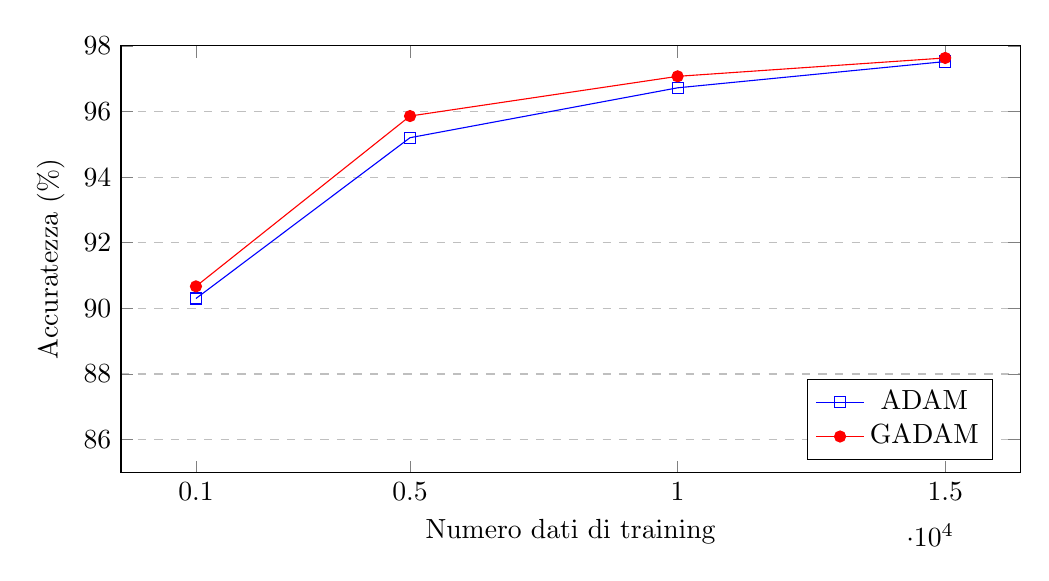
\begin{tikzpicture}
    \begin{axis}[
        width=13cm,
        height=7cm,
        xlabel={Numero dati di training},
        ylabel={Accuratezza (\%)},
        ymin=85, ymax=98,
        xtick={1000,5000,10000,15000},
        legend pos=south east,
        ymajorgrids=true,
        grid style=dashed
    ]
    
    % ADAM
    \addplot[
        color=blue,
        mark=square
    ] coordinates {
        (1000,90.30) (5000,95.2) (10000,96.72) (15000,97.52)
    };
    \addlegendentry{ADAM}
    
    % GADAM
    \addplot[
        color=red,
        mark=*
    ] coordinates {
        (1000,90.67) (5000,95.86) (10000,97.07) (15000,97.63)
    };
    \addlegendentry{GADAM}
    
    \end{axis}
    \end{tikzpicture}
    \caption{Accuratezza di ADAM vs GADAM al variare della dimensione del dataset}
    \end{figure}
    